\chapter{Discourse Marker Insertion}

\label{Chapter05}

\section{Problem}

Discourse markers are words or phrases which function to organize speech, by segmenting it, defining relationships between sections, and generally allowing a text to ``flow''. Despite their technically vague semantics and lack of a defined grammatical purpose (they can also be referred to as ``fillers''), they play an important linguistic part in both conversation and written speech.

As shown empirically both in this project (Table \ref{acro-edits-table}) and in previous literature (Table \ref{pavlick2016table}), discourse markers can be found in informal language, where they do not appear in formal language. A complete list of the discourse markers extracted from the informal side of the Acrolinx blog posts data is in Appendix \ref{Appendix01}. 

When entering a discussion on why these markers are present in informal language, it should be noted that the list in Appendix \ref{Appendix01} is not exhaustive. For example, ``nevertheless'', which is a discourse marker but certainly also formal, does not appear. Therefore, this problem inherently has a lexical component. Still, the definite and significant presence of at least these discourse markers in informal language invites these studies.

Discourse markers are likely regarded as informal in part because of their semantic vacuity: as discussed, formal language aims to be precise and absent of any so-called ``fuzzy'' terms. ``So there you have it'' --- where is ``there''? What is ``it''? Even with context, these things may not be immediately clear. The more surface-level, stylistic aspect of formality also comes into play here. In English grammar classes students are often prescriptively taught not to begin sentences with conjunctions, which would introduce a bias against discourse markers as ``but'' or ``and'' in speech that is meant to be more correct.

Following the pattern set by the edits categorized in the Acrolinx Blog Post Dataset, I focused on discourse markers which appear at the beginning of a sentence. This makes them easy to identify --- mid-sentence, some markers could be confused with other parts of speech, like ``now'' or ``first''. In any case, identifying and removing these markers from the beginnings of sentences is a fairly trivial task, perhaps able to be accomplished with lexicons alone. On the other hand, placing discourse markers in sentences is a different and certainly more difficult goal. ``But'' or ``so'' cannot be simply added to any sentence --- though the sentences can survive without them, they do signal an important relation between what has come before, and what is coming next. Even ``oh'', perhaps one of the simplest included markers, is interesting enough to inspire whole papers, and might signal some peripheral but still relevant information, or indicate an attempt to move a discussion forward (\cite{bolden2006oh}).

So, the insertion of discourse markers requires context, and both semantic and syntactic information. The resulting question to handle this problem became: given two consecutive sentences, can a particular discourse marker be inserted at the beginning of the second sentence? This gives both preceding and succeeding context to determine the potential presence of a marker.

I selected the most common nine discourse markers from the list in Appendix \ref{Appendix01}, based on the availability of data. Then, I trained a model for each of them to predict that marker's possible insertion in the sentence. Results were generally promising, though they seem to overpredict on out-of-domain data; increasing the softmax threshold works well in addressing this problem, though. In this chapter, I report on the data gathered, experiments developed and end results of this approach to the problem of (selective) discourse marker insertion.

\section{Data}

When compiling a dataset for this task, two main sources were used: the British National Corpus (BNC) (\cite{bnc}) \footnote{Data cited herein have been extracted from the British National Corpus, distributed by the University of Oxford on behalf of the BNC Consortium. All rights in the texts cited are reserved.} and the Open American National Corpus (\cite{ide2001oanc}). All texts were extracted and split into sentences. Only the texts from the OANC's spoken categories were skipped from then on, as they included no capitalization and included a high proportion of sentences of length 5 or less. 

\subsection{Sentence Pairs}

For each discourse marker, sentences in which that marker could be found at the start of the sentence (barring punctuation such as quotation marks) were extracted, along with the sentence preceding it. If there was no preceding sentence, the example was passed over; that context would be crucial to the experiment. I initially computed which discourse markers appeared most frequently in the data, and chose to focus on only those which had more than 1000 available samples.

Next, some special cases wherein the sentence could not stand without the discourse marker, or it was not a discourse marker at all, were removed. These included sentences that began with ``Now that'', ``First of all'' or ``So much that'', in which removing the word would have created a bad sentence. Pairs with sentences of length less than 3 were also removed.

Finally, the discourse markers were removed from the sentences, and the appropriate new first word capitalized in its place. A label was given to the sentence pair for the marker that was removed. If no discourse marker was present, the sentence pair was also given a corresponding label.

\begin{table}[h]
\centering
 \begin{tabular}{|| p{5.5cm} | p{5.5cm} | p{1cm} ||} 
 \hline
 First Sentence & Second Sentence & Label \\ [0.3ex] 
 \hline\hline
 Remember that scene in ``Sleeper'' where it's revealed that in the future everybody knows the only really healthy substances are red meat and cigarettes? & 
    Today's WP runs a story headlined ``Smoking May Protect Some High-Risk Women from Breast Cancer.'' &
    Well \\
\hline
 The paper points out that the episode is apt to rekindle consumer concerns about online credit card security. & 
    Since the jerkball's e-mail trail leads to eastern Europe, the case stands to highlight the freedom online criminals have to operate beyond U.S. jurisdiction. &
    Also \\
\hline
 In his shambling gait and glassy, uncertain stare he reminds me all too closely of another awesome wreck of a man who led another awesome wreck of a country: Marshall von Hindenburg at the end of his life. & 
    That scares me, because the similarities between Hindenburg's Weimar Germany and Yeltsin's Russia seem all too exact. &
    And \\
\hline
\end{tabular}
\caption{Examples of sentences with labels from the data compiled from the OANC and BNC.}
\label{disc-mark-data-examples}
\end{table}

The result was a dataset of tokenized sentence pairs, with discourse markers removed, and each one attached to a label of a specific marker or a label for no marker at all. A few examples are given in Table \ref{disc-mark-data-examples}.

\subsection{Vectorization}

I used doc2vec to vectorize each of the two sentences. Doc2vec trains an unsupervised model to learn feature representations of a predetermined length from variable-length text (\cite{le2014doc2vec}). I trained the model through a Python package called gensim (\cite{rehurek2010gensim}). With this method, not only can individual word information be encapsulated in output vectors, but syntactic relationships can also have an effect on the outcome.

I trained a doc2vec model on all sentences from the OANC and the BNC for 20 epochs, in order to produce 100-dimensional output vectors for each sentence. Final representation, therefore, was a sequence of two 100-dimensional doc2vec embeddings.

\subsection{Final Dataset Statistics}

\begin{table}[h]
\centering
 \begin{tabular}{|| l | r | r ||}
 \hline
 Data Subset & Number & \% \\ [0.3ex] 
 \hline\hline
 Total & 835,350 & --- \\
 \hline
 OANC & 273,702 & $32.8\%$ \\
 \hline
 BNC & 273,702 & $67.2\%$ \\
 \hline
 No Discourse Marker & 785,192 & $94.0\%$ \\
 \hline
 Discourse Marker & 50,158 & $6.0\%$ \\
 \hline
\end{tabular}
\caption{A numeric overview of the data on discourse markers compiled from the OANC and BNC corpora.}
\label{disc-mark-gen-data-stats}
\end{table}

Unsurprisingly, in the end there were far more examples without discourse markers in the original sentences than examples with them. An overview of the proportions of non-discourse marker sentence pairs versus sentence pairs with discourse markers removed, as well as how much data came from the BNC as opposed to the OANC, is presented in Table \ref{disc-mark-gen-data-stats}.

\begin{table}[h]
\centering
 \begin{tabular}{|| l | r ||}
 \hline
 Term & \# Examples \\ [0.3ex] 
 \hline\hline
 But & 21392 \\
 \hline
 And & 12918 \\
 \hline
 So & 4740 \\
 \hline
 Now & 2466 \\
 \hline
 Well & 2279 \\
 \hline
 Yet & 1909 \\
 \hline
 First & 1636 \\
 \hline
 Or & 1606 \\
 \hline
 Also & 1212 \\
 \hline
\end{tabular}
\caption{The number of examples for each removed discourse marker from the OANC/BNC data, from most to least.}
\label{disc-mark-dm-stats}
\end{table}

The original dataset was large enough that the resulting number of data points for each discourse marker were still substantial, particularly for the most common markers. The list of final chosen discourse markers to be used in these experiments, plus the number of samples labeled for each one, is given in Table \ref{disc-mark-dm-stats}. 

\section{Methods}

I trained a separate model for each discourse marker, on separate datasets extracted from the compilation described above. Therefore, the task was binary classification for each pair of sentences: could this discourse marker be inserted here, yes or no?

One could argue that a better methodology would be multi-class classification, wherein a single model predicts which of a list of discourse markers, if any, best fits between sentences. This was decided against for multiple reasons. Firstly, there is no reason why multiple discourse markers could not be a good fit for a given pair of sentences, if they share some contexts in which they are likely to appear (for example, ``and'' and ``also'', or ``now'' and ``so''). And secondly, the disparity in amount of data between discourse markers, as shown in Table \ref{disc-mark-dm-stats}, meant that creating a balanced dataset would either involve oversampling many times from the smaller terms, or subsampling from the terms with more data and thereby losing most of the potential samples. To encapsulate this potential of multiple discourse markers to appear in the same spot, and to fully take advantage of the terms which appeared more often in the data, I chose to train separate models.

\subsection{Architecture}

\begin{figure}
    \centering
    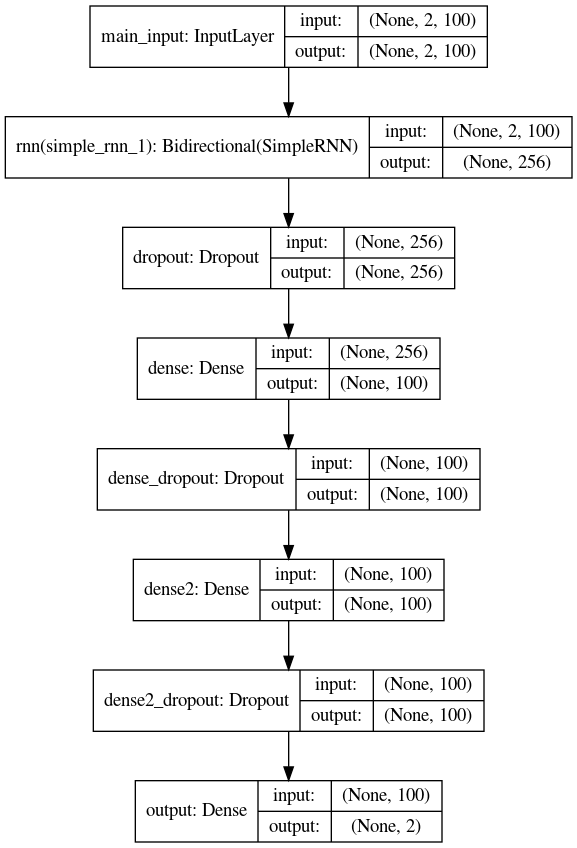
\includegraphics[width = 10cm]{Figures/graph.png}
    \caption{Visualization of the architecture for the models used to train for the discourse marker insertion task. Note that ``None'' represents the batch size.}
    \label{fig:disc-mark-architecture}
\end{figure}

The same architecture, developed using keras with tensorflow backend, was used to train all nine models (\cite{chollet2015keras}). It includes a bidirectional recurrent neural network (RNN) with 128 units followed by a dropout layer. After that there are two fully-connected layers with 100 units each and using rectified linear units (ReLU) for activation, each also connected to a dropout layer. Finally, there is a softmax output layer. The dropout rate is set to 0.5 for all relevant layers. Models are compiled with AdamOptimizer and the loss function is set to binary cross-entropy loss. A simple graph of the architecture with input and output shapes can be found in Figure \ref{fig:disc-mark-architecture}.

Hyperparameter optimization of the dropout rate and number of units for the RNN and the dense layers was carried out over the largest validation set, that of ``But'', and then kept constant for the models of the other discourse markers. The choice was made to not due individual hyperparameter optimization for each discourse marker due to the small dataset sizes of most of the others.

\subsection{Training}

\begin{table}[h]
\centering
 \begin{tabular}{|| l | r | r | r ||}
 \hline
 Term & train & val & test \\ [0.3ex] 
 \hline\hline
 But & 34655 & 3850 & 4278 \\
 \hline
 And & 20926 & 2325 & 2584 \\
 \hline
 So & 7678 & 853 & 948 \\
 \hline
 Now & 2995 & 443 & 493 \\
 \hline
 Well & 3690 & 410 & 456 \\
 \hline
 Yet & 3091 & 343 & 382 \\
 \hline
 First & 2650 & 294 & 327 \\
 \hline
 Or & 2601 & 289 & 381 \\
 \hline
 Also & 1963 & 218 & 242 \\
 \hline
\end{tabular}
\caption{The sizes of each training, validation and test set for the chosen discourse markers.}
\label{disc-mark-train-tune-test}
\end{table}

For each term, all the samples with the appropriate label were collected, and then a balanced dataset was compiled by randomly sampling the same number of instances from the data that had no discourse markers. Datasets were shuffled and then separated into train and test at a split of 0.9/0.1, and then the resulting training set was split into final train and validation at the same split of 0.9/0.1. This was done using the popular toolkit scikit-learn (\cite{scikit-learn}). Final lengths for training, validation and test sets are given in Table \ref{disc-mark-train-tune-test}. Some of these data subsets are quite small, and this should be kept in mind as we move on to look at results.

All models were trained for 5 epochs over their respective datasets with batch size 32. Training was very quick, with the largest set (``But'') taking only 8 seconds per epoch.

\section{Results}

Having nine different models with nine different dataset sizes means there are a substantial amount of numbers to keep track of. In this section I present quantitative results together with any overall trends or primary takeaways.

\subsection{Test Accuracy}

\begin{table}[h]
\centering
 \begin{tabular}{|| l | r | r | r | r ||}
 \hline
 Term & test-accuracy & precision & recall & f1-score \\ [0.3ex] 
 \hline\hline
 But & $76.5$ & $84.9$ & $64.2$ & $73.1$ \\
 \hline
 And & \color{red}{$78.6$} & $85.4$ & \color{red}{$70.8$} & \color{red}{$77.4$} \\
 \hline
 So & \color{red}{$77.1$} & \color{red}{$87.5$} & \color{blue}{$63.4$} & \color{red}{$73.5$} \\
 \hline
 Now & $75.5$ & $79.6$ & $65.0$ & $71.5$ \\
 \hline
 Well & \color{red}{$85.5$} & \color{red}{$91.9$} & \color{red}{$79.8$} & \color{red}{$85.5$} \\
 \hline
 Yet & $72.0$ & \color{blue}{$74.1$} & $66.7$ & \color{blue}{$70.2$} \\
 \hline
 First & \color{blue}{$69.4$} & \color{red}{$93.8$} & \color{blue}{$49.2$} & \color{blue}{$64.5$} \\
 \hline
 Or & \color{blue}{$70.7$} & \color{blue}{$67.2$} & \color{red}{$76.0$} & $71.3$ \\
 \hline
 Also & \color{blue}{$57.4$} & \color{blue}{$62.8$} & \color{blue}{$43.2$} & \color{blue}{$51.2$} \\
 \hline
\end{tabular}
\caption{Important evaluation metrics for the test sets, with the model trained for each term. The three highest scores for each metric are colored red; the three lowest are colored blue.}
\label{disc-mark-test-results}
\end{table}

The metrics used to evaluate the models were accuracy, precision, recall and f1-score. These metrics carried out on the test set for each model are given in Table \ref{disc-mark-test-results}. For each metric, the highest three scores are colored red, and the lowest three are colored blue. Overall, ``And'', ``So'' and ``Well'' had the best results, while ``First'', ``Or'' and ``Also'' performed the worst. Notably, all models except for that of ``Or'' had significantly better precision than recall. 

Note that the order the terms are presented in is preserved from Tables \ref{disc-mark-gen-data-stats} and \ref{disc-mark-data-examples}: descending order of dataset size. This provides additional context to our better- and worse-performing models: the models of those terms, which were trained on the least data (in all three cases less than 3000 training samples), struggled the most. This is likely to be an important reason for their performance.

\subsection{Training Accuracy}

\begin{table}[h]
\centering
 \begin{tabular}{|| l | r | r | r ||}
 \hline
 Term & train-during & train-after & validation \\ [0.3ex] 
 \hline\hline
 But & $75.0$ & \color{red}{$77.1$} & $76.2$ \\
 \hline
 And & $75.2$ & \color{red}{$78.9$} & $76.9$ \\
 \hline
 So & $72.2$ & \color{red}{$77.4$} & $75.6$ \\
 \hline
 Now & $66.8$ & \color{red}{$72.4$} & $67.1$ \\
 \hline
 Well & $81.6$ & \color{red}{$85.5$} & $84.7$ \\
 \hline
 Yet & $70.9$ & \color{red}{$74.6$} & $70.1$ \\
 \hline
 First & $70.5$ & \color{red}{$72.6$} & $70.8$ \\
 \hline
 Or & $74.1$ & \color{red}{$78.0$} & $75.2$ \\
 \hline
 Also & $63.1$ & \color{red}{$69.5$} & $66.2$ \\
 \hline
\end{tabular}
\caption{The resulting accuracy for the model of each term, over their training set while training happened (thus with dropout), and over both training and validation sets with the full number of units active. In all cases, the training accuracy given all active units is the highest (marked in red).}
\label{disc-mark-train-acc}
\end{table}

In this case, accuracy over the training set provides additional relevant information. In Table \ref{disc-mark-train-acc}, training and validation accuracy results are displayed. Two scores over the training set are actually given, the first, crucially, calculated during training, and the second in evaluation mode after training is over. For the most part, the accuracy results from during training are lower than the test accuracy results --- and this would be unexpected behavior for the model. However, this does not take into account that during training, accuracy is calculated by evaluating on the model with dropout. In the architecture presented here, with a dropout rate of 0.5, this could be a model with half of its units deactivated. The accuracy over the training set after training is complete is appreciably higher for all discourse markers. 

It should also be noted that this training accuracy and the test accuracy are fairly close in most cases. This suggests that the dropout rate has done its job of regularization: that the models were able to generalize to the test data. The only exceptions thereof are with the two models with the least data, ``Or'' and ``Also'', which performed significantly worse on the test data. These models were likely not able to generalize so well regardless of any regularization methods simply due to this lack of training information.

\section{Discussion}

Quantitative results alone cannot give us a good picture of what, exactly, the models are doing right and wrong. In this section I focus the discussion on error analysis, supported by qualitative data in the form of individual examples. In the interests of brevity, I will not go deep into the differences between the discourse markers, but will instead stick to overall patterns among them. 

\subsection{Noise in Negative Data}

The method of dataset collection here has left a problem. The data used to train these models was collected from real texts. The issue is that authors naturally do not always use these discourse markers where they \textit{could} be used. Therefore, while the positive samples (those which had the discourse marker originally) are definite cases of where the marker could go, the negative samples might have some data that are actually positive. A look at the negative training data confirms this:

\begin{quote}
\small{SENTENCE 1:} \quad The local authority served on the defendant written demands for the expenses they had incurred in respect of the works required under the notices, respectively on 31 May 1984 and 25 April 1985. \linebreak
\small{SENTENCE 2:} \quad \small{[NULL]} The defendant did not pay. 
\end{quote}

This was a negative sample for ``And''; however, ``And'' could still sensibly, perhaps even naturally, appear at the beginning of the second sentence. Interestingly, so could ``But'' --- further supporting the idea that while the two words might have opposing definitions as conjunctions, as discourse markers their differences are less clearly defined. Regardless, this form of noise in the data has two consequences: first, it would make it more difficult for models to learn what clearly separates a sentence which can take the marker from a sentence which cannot. Secondly, from what the model \textit{has} generalized, it may assign a positive label to a pair of sentences which could plausibly take the discourse marker, but which in the original data did not have it. 

Such is the case in the following example:

\begin{quote}
\small{SENTENCE 1:} \quad Their discord provided accompaniment for the chase that now developed between the two beings. \linebreak
\small{SENTENCE 2:} \quad \small{[true: NULL][pred: First]} She darted round and round the tower, running fast but waving her hands. 
\end{quote}

The original label was not ``First'', but the model predicted its presence. And in this case, ``First'' is a reasonable insertion for this pair of sentences.

Given this assumption of noise but only in the negative data, however, one might expect higher recall than precision. That is, the models, having generalized properly, would pick up not only all of the correctly labeled positive examples, but also all of the negative examples which could, in fact, take the discourse marker in question. Actually, though, the effects of the noise could be seen on precision and recall the other way, as well. The models may have also picked up in training on the improperly labeled negative data and thus tended to underpredict. It is difficult to separate out these two possibilities without having the entire dataset validated by humans.

\subsection{Lack of Context}

The other form of noise in the dataset has to do with the restricted context window. Two sentences were kept for each data point: the sentence which could have the discourse marker at its start, and the sentence immediately before it. This provides some context about the point the text is trying to make, the conversational place those sentences are at, and the logical progression of ideas. However, it naturally does not give all of that context. In some cases, these two sentences may not be enough. Consider:

\begin{quote}
\small{SENTENCE 1:} \quad I am glad that you talked to Ken Arrow.
\linebreak
\small{SENTENCE 2:} \quad \small{[true: But][pred: NULL]} Nobel laureates, who have wide responsibilities and much on their mind, are not necessarily on top of what has been going on in research outside their usual field.
\end{quote}

With these two sentences alone, one does not know anything about Ken Arrow, and what point the second sentence might be trying to make. Perhaps Ken Arrow is the busy and as such potentially uninformed Nobel laureate (for the record: he is), or perhaps a questioner failed to find their answer with another Nobel laureate, and then went to Ken Arrow for another opinion. Additional context could have made this placement more precise.

\subsection{Doc2Vec Issues}

The idea behind representing each sentence using doc2vec, instead of a sequence of word2vec embeddings, was that the syntactic and semantic information of each sentence would be contained in its vector. Then, when processing a series of sentences, the relationship between those sentences could be more clearly identified. Nevertheless, this method comes with its own disadvantages. Compressing, for example, a sequence of 20 word vectors, each with 100 dimensions, into a single 100-dimensional sentence vector, naturally means potential loss of important information --- particularly when that important information lies in a single word.

\begin{quote}
\small{SENTENCE 1:} \quad December is already an unkind month for those of us with combination skin .
\linebreak
\small{SENTENCE 2:} \quad \small{[true: But][pred: NULL]} On this third day of latkes, many of us awoke to find that our faces haven't been this splotchy since our bar mitzvahs.
\end{quote}

Whether or not ``But'' can be placed in this second sentence hinges on a single word in the first sentence: ``already''. With that word, placing that discourse marker is an option: this month is \textit{already} bad, and then something happened to make it \textit{worse}. Without it, though, the second sentence with ``But'' falls apart, as it then implies something nice about December should be coming, which is undoubtedly not the case. It is possibly the most important word for this problem in these sentences, and it may be that the doc2vec encoding causes its presence to be lost. Here is another example:

\begin{quote}
\small{SENTENCE 1:} \quad Quantitative methods were incorporated in the case study in two ways.
\linebreak
\small{SENTENCE 2:} \quad \small{[true: NULL][pred: First]} The first was in triangulation: the use of several forms of data within a single case study in order to give many reference points for verifying patterns and ruling out alternative explanations in order to achieve what evaluators call ``internal validity.''
\end{quote}

Here, there is a clear redundancy with the predicted insertion of ``First.'' If ``the first'' was not already there --- if, for example, it were replaced by ``one method was'' --- then the prediction would make sense. Instead of the overall semantic meaning and relationship of the sentences determining a prediction, it is both those overall characteristics \textit{and} the presence of a couple of important words which are most important. And again, when this (longer) sentence was transformed into a 100-dimensional vector, it is possible that a significant enough signal for the presence of those particular words was lost.

\subsection{Practical Usage: Microsoft Example}

Since an original problem with the GYAFC corpus and subsequent trained models was that it was too informal and did not translate well to out-of-domain data, specifically the Microsoft Azure corpus, it is helpful to try out these models on example text from those data. Ideally, when applying all these models to a text, key discourse markers would be suggested in certain places, helping the text to overall become more informal or conversational. Below is a sample passage from the corpus, with suggested insertions from all nine models given (\cite{microsoft2019azure}):

\begin{quote}
The Azure portal is a web-based, unified console that provides an alternative to command-line tools. \textbf{[Now/Also/And]} With the Azure portal, you can manage your Azure subscription using a graphical user interface. \textbf{[But/And]} You can build, manage, and monitor everything from simple web apps to complex cloud deployments, create custom dashboards for an organized view of resources, and configure accessibility options for the best experience. \textbf{[First/But/And]} The Azure portal is designed for resiliency and continuous availability. \textbf{[First/Now]} It has a presence in every Azure datacenter thereby making it resilient to individual datacenter failures and also avoids network slow-downs by being close to users. \textbf{[So/Also]} The Azure portal updates continuously and requires no downtime for maintenance activities.
\end{quote}

If these were suggestions to an author in order to make their text less formal, it might be too much. The models are overpredicting for this use case: there are too many suggestions, for too many of the sentences in a single paragraph. It is unhelpful as guidance for a writer.

Having softmax output gives us an easy way to tweak this, though. Often, the argmax function is used over the softmax output, meaning that if the probability of ``And'' being present is .51 and the probability of it not being present is .49, a positive prediction is given. By raising that threshold, one can ensure that the model predicts the positive class only when it has a higher degree of certainty as to its presence.

I raised the threshold to a probability of 0.75 to get the following output:

\begin{quote}
The Azure portal is a web-based, unified console that provides an alternative to command-line tools. \textbf{[And]} With the Azure portal, you can manage your Azure subscription using a graphical user interface. You can build, manage, and monitor everything from simple web apps to complex cloud deployments, create custom dashboards for an organized view of resources, and configure accessibility options for the best experience. \textbf{[And]} The Azure portal is designed for resiliency and continuous availability. It has a presence in every Azure datacenter thereby making it resilient to individual datacenter failures and also avoids network slow-downs by being close to users. \textbf{[So]} The Azure portal updates continuously and requires no downtime for maintenance activities.
\end{quote}

These predictions are fewer, more correct, and more concrete. They would provide more useful guidance to a writer who wants their text to be less formal.

\section{Future Work}

First and foremost, work could be done to clean any noise from the automatically gathered dataset. Manual validation would, naturally, be ideal. However, even if that is not possible, there are more steps that could be taken to reduce noise. For example, to compile negative samples for each model, instead of randomly sampling from the null case and all other discourse markers, one could sample only from the data for a discourse marker that tends to appear in different contexts. Examples might be ``But'' and ``First'', or ``Also'' and ``Or''. More research would be required to precisely delineate these patterns.

In general, more data from other corpora could be added, particularly for those discourse markers which had very small training sets. Given more data, it would be interesting to revisit the possibility of approaching this problem as a multi-class classification task, wherein the question becomes which discourse marker among a set could be placed in a particular sentence.

Next, more context could be added to the instances: instead of just a sentence pair, a series of sentences in a paragraph could all be vectorized to a sequence, with a mask to mark the potential location of the discourse marker. This could provide the necessary context to decide with more certainty if a certain marker can truly be inserted in a location, based on the overall content of the paragraph.

As discussed, doc2vec has advantages and disadvantages both. Directly comparing its usage with that of sequenced word vectors would provide useful insight and perhaps even turn out an improvement in performance.

And finally, other architectures could be experimented with. Transformers, which eschew recurrence entirely in favor of attention, could be a worthwhile avenue to explore for this task.

\section{Takeaway}

In general, this problem revealed itself to be trickier than it first seemed. There is ambiguity in many potential placements, and more context than expected turns out to be necessary in order to make precise predictions. Although the automatically formed dataset served its purpose well enough, future work would need to start with reducing its noise. 

Of course, in the end the purpose of attempting this task was to assist in the overall goal of making texts more informal. That brings us to the necessity of translating the question of ``Could this discourse marker go here?'' to ``Should an author add this discourse marker here, to make their text more informal?'' Adapting the models developed in this chapter to a practical usage would require further research. Nonetheless, results overall are promising, and could be extended for this purpose.